\section{Specifications}
\label{sec:Specifications}

\newcounter{rulei}[subsection]
\newcommand{\rcnii}{\stepcounter{rulei}\arabic{section}.\arabic{subsection}.\arabic{rulei}}
\renewcommand{\labelenumi}{\rcnii}

\subsection{Markers}
\label{sub:markers}
The arena, tokens, slots, and robots involved in the game are labelled with \textit{libkoki} markers.
Each marker pattern encodes a number.
Each marker number is associated with a particular feature within the arena, and also has an associated size.
The marker numbers and sizes are as follows:

\begin{center}
  \begin{tabular}{lcc}
    \toprule
    \textbf{Item} & \textbf{Marker Numbers} & \textbf{Marker Size (mm)} \\
    \midrule
    Arena boundary & {} 0 -- 27 & 250 \\
    Robots & 28 -- 31 & 100 \\
    Slots & 32 -- 39 & 160 \\
    Token Top & 40 -- 43 & 160 \\
    Token Bottom & 44 -- 47 & 160 \\
    Token Side & 48 -- 51 & 160 \\
    \bottomrule
  \end{tabular}
\end{center}

Two sets of marker codes will be used: one for development purpose, and one for the competition itself.
The competition set is only to be used inside the Student Robotics arena at the Student Robotics competition.
This is so that people carrying markers past the arena do not confuse robots.
The competition codes are 100 above the development codes.
When run in competition mode (specifiable through the robot's GUI), the software provided by Student Robotics will subtract 100 from the detected marker codes, as well as ignore the development codes.

The markers can be printed on a black-and-white printer.
Marker designs can be downloaded from the documentation section of the Student Robotics website.

Unless specified otherwise, all markers described in this document are oriented vertically such that the principle corner of the marker (which is indicated by a dark grey dot in the black marker border) is on the higher edge.

\subsection{Robot Badges}
\label{sec:robot-badges}

\begin{figure}
  \centering
  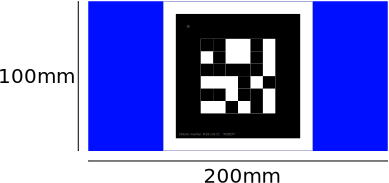
\includegraphics[width=\textwidth]{./images/robot-marker.pdf}
  \caption{An example robot badge.
           The blue areas shown are the human-compatible areas.
	   All dimensions are in millimetres.}
  \label{fig:example-badge}
\end{figure}

\begin{enumerate}
\item A ``robot badge'' is a removable identifier that will be attached to a robot throughout a match.
      It features the robot's assigned marker for the match, as well as human-compatible areas to allow spectators to easily associate a robot with its starting location.
      An example of one of these badges is shown in figure~\ref{fig:example-badge}.
      The markings in the human-compatible areas are intentionally not specified.

\item A robot must feature four of the badge mounts shown in figure~\ref{fig:badge-mounting}.
      These mounts must permit a flat $200 \times 100mm$ panel to be attached to them.
      The three areas of each mount must feature the illustrated areas of hook-type Velcro to allow this panel to be fitted.

\item The four badge mounts must be on the exterior of the robot, parallel with the vertical plane, and should be perpendicular to each other about the vertical axis\footnote{Teams can apply for a team-specific rule alteration to the required number of badges.
      Clear justification must be provided by the team with such a request.}
      The orientation of the badge mounts is unimportant, but teams are encouraged to position them horizontally as shown in figure~\ref{fig:example-badge}.

\item The mapping between a given robot and its robot badge is as follows:

\begin{center}
  \begin{tabular}{cc}
    \toprule
    \textbf{Corner} & \textbf{Marker Number} \\
    \midrule
    0 & 28 \\
    1 & 29 \\
    2 & 30 \\
    3 & 31 \\
    \bottomrule
  \end{tabular}
\end{center}

\begin{figure}
  \centering
  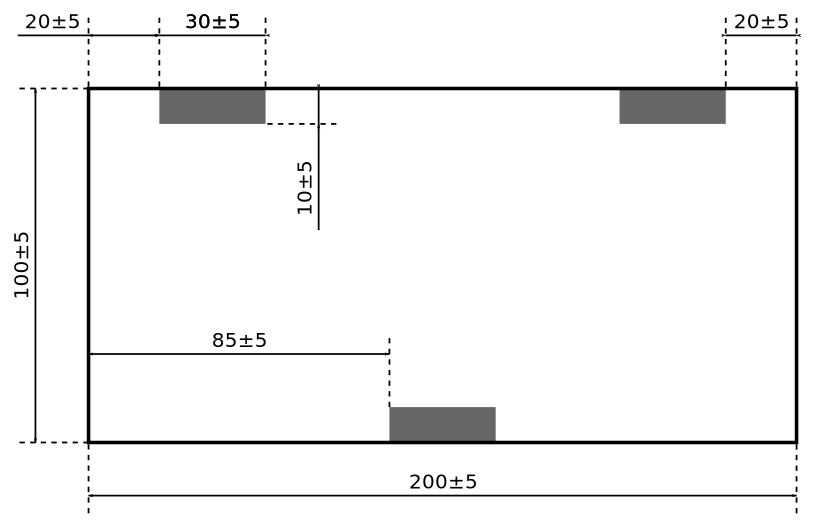
\includegraphics[width=\textwidth]{./images/badge-mounting.pdf}
  \caption{The dimensions of the required robot badge mountings.
           The shaded areas are hook-type Velcro.
           All dimensions are in millimetres.}
  \label{fig:badge-mounting}
\end{figure}

\end{enumerate}

\subsection{Arena}
\label{sub:arena}
\begin{enumerate}
\item The match arena floor, overall, is an $8m \times 8m$ square, as shown in figure~\ref{fig:arena-dim}.
      The tolerance of these two dimensions is $\pm0.25m$.

\begin{figure}
  \centering
  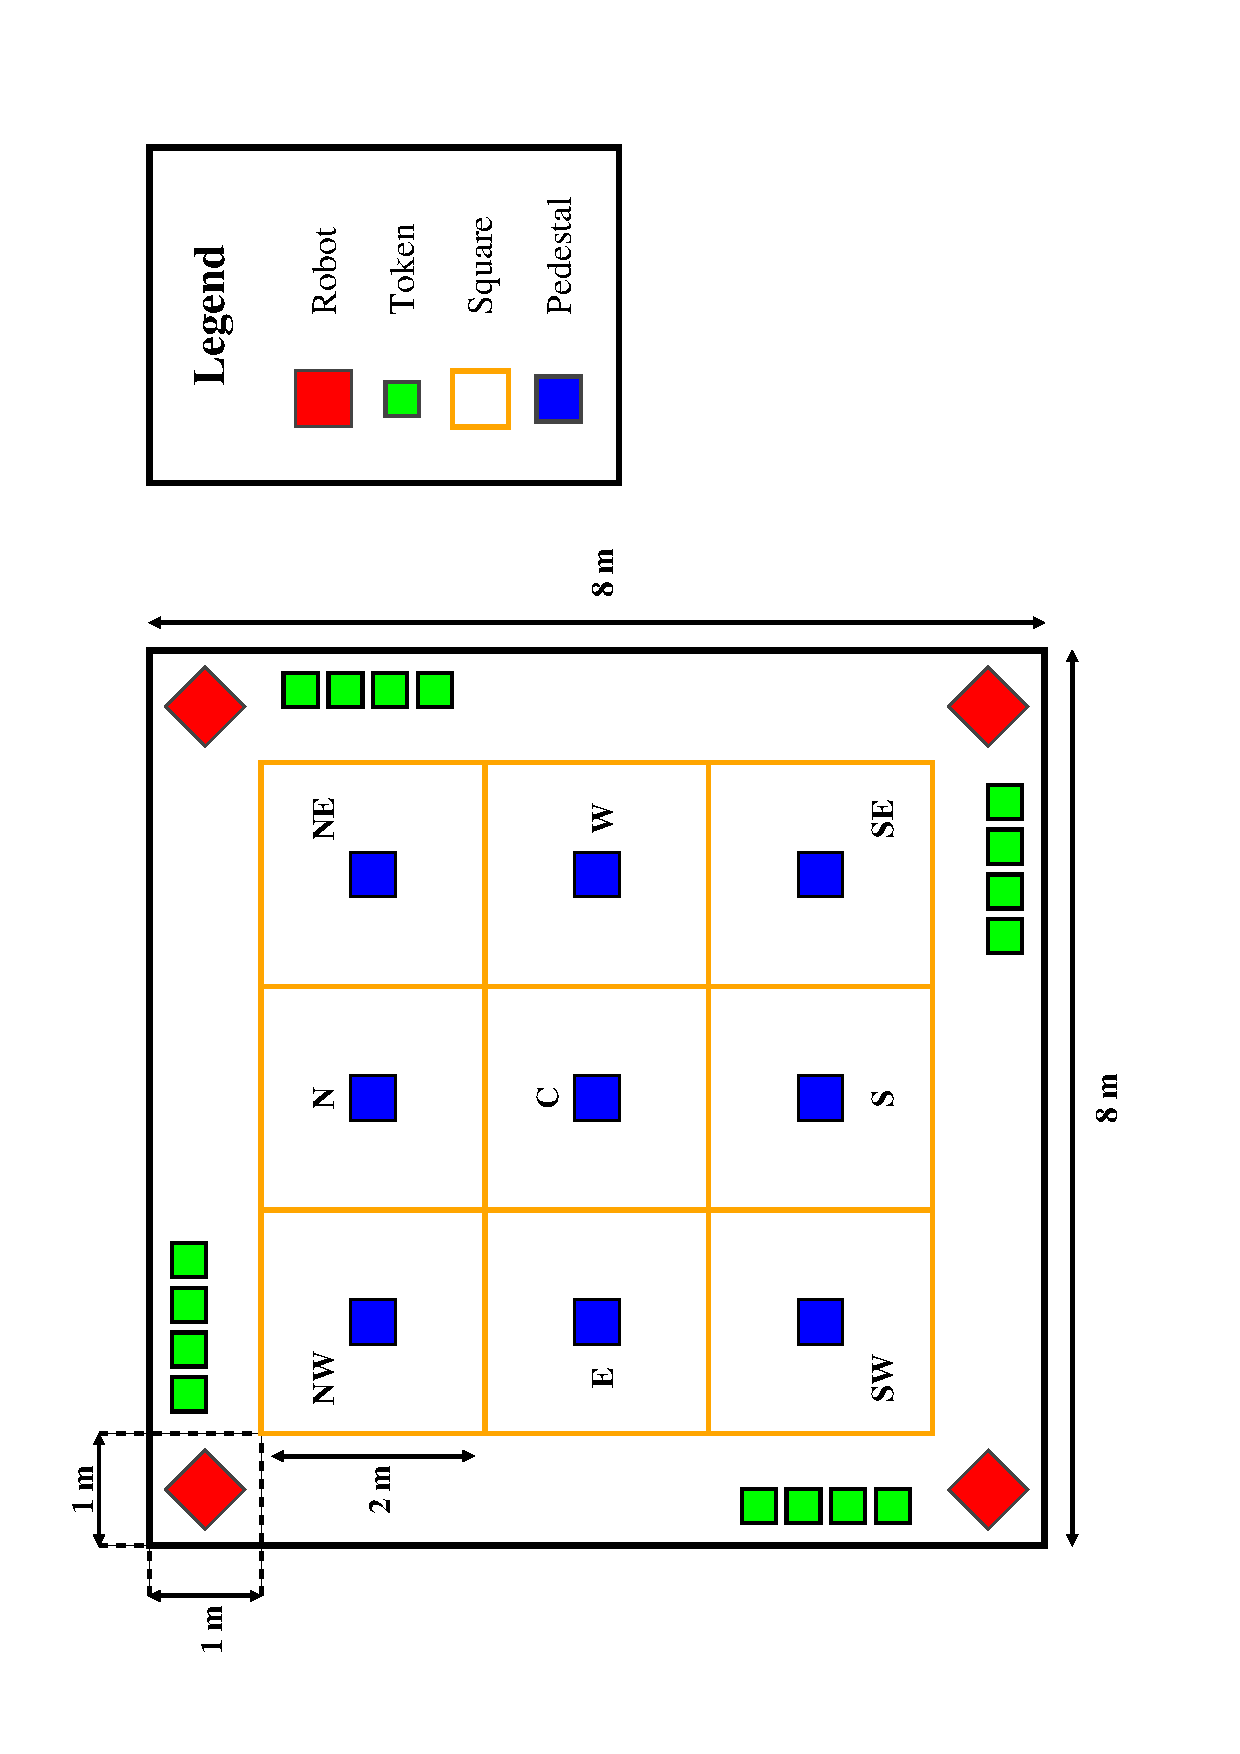
\includegraphics[width=\textwidth]{./images/arena.pdf}
  \caption{\label{fig:arena-dim}A bird's-eye view of the arena. All dimensions are in millimetres.}
\end{figure}

\item The floor of the arena is covered with a closed-loop, short pile carpet.

\item The arena walls are $600\pm30mm$ high, the interior surfaces of which are white plastic-coated hardboard.

\begin{figure}
  \centering
  
\includegraphics[width=\textwidth]{./images/sidewall.pdf}
  \caption{Seven $250mm$ wide markers are spaced evenly along each $8m$ arena wall.
           The markers are placed $50mm$ above the floor.
	   All dimensions are in millimetres.}
  \label{fig:arena-wall}
\end{figure}

\begin{figure}
  \centering
  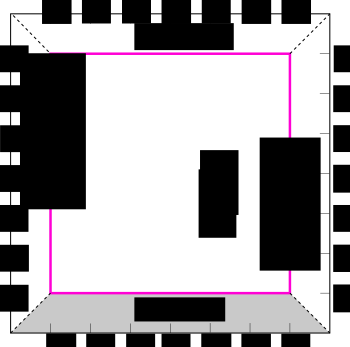
\includegraphics[width=0.5\textwidth]{./images/arena-markers.pdf}
  \caption{Twenty eight arena wall markers are positioned around the perimeter of the arena with the marker codes incrementing in a clockwise fashion.
           Eight slot markers are incremented from number 32, in an anti-clockwise fashion around the zones.
           The corners are counted in a clockwise fashion, with corner 0 being the corner closest to arena marker 0.}
  \label{fig:arena-zones}
\end{figure}

\item Each wall of the arena features seven $250mm$ libkoki markers.
      Figure~\ref{fig:arena-wall} shows the positioning of these markers, whilst figure~\ref{fig:arena-zones} shows the numbering of these markers.

\item Each robot will be assigned a corner at the start of every match to indicate its starting position.
      Corner starting positions are $1000 \pm 20mm$ square and will be marked by $25mm$ paper-based masking tape.
      The mapping of these corner numbers in the arena is shown in figure~\ref{fig:arena-zones}.

\item Student Robotics reserves the right to have up to three match officials in the arena during games.

\end{enumerate}


\subsection{Zones}
\label{sub:Zones}

\begin{figure}
  \centering
  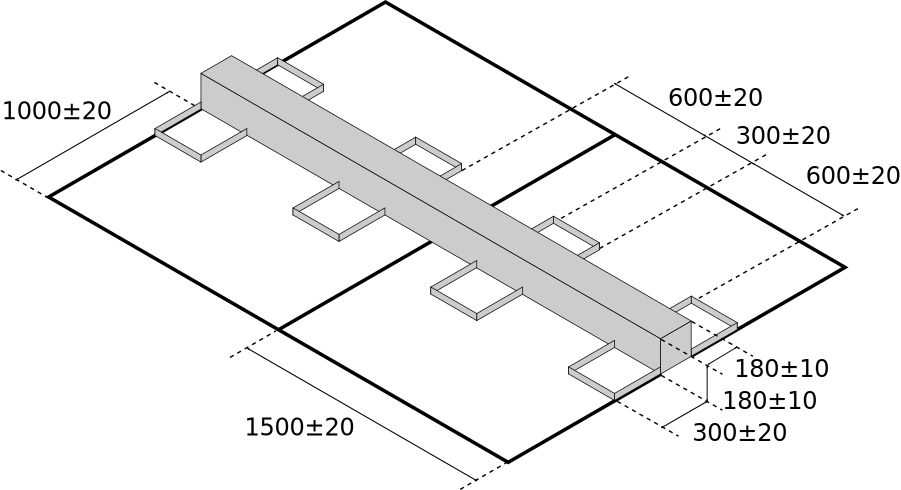
\includegraphics[width=\textwidth]{./images/slots-zones.pdf}
  \caption{The arena contains four zones, each $1500 \pm 20mm$ wide and $1000 \pm 20mm$ deep.
           The rectangle described by the four zones is split in two by a $180 \pm 10mm$ high, $180 \pm 10mm$ deep zone wall.
           Eight $25 \pm 5mm$ high slots---two in each zone---are attached to the zone wall.
           All dimensions are in millimetres.}
  \label{fig:slots-zones}
\end{figure}

\begin{enumerate}
\item There are four zones in the centre of the arena.
      The arrangement of these zones can be seen in figure~\ref{fig:arena-dim}, and is shown in more detail in figure~\ref{fig:slots-zones}.

\item Each zone is $1500mm$ wide and $1000mm$ deep and is  marked with $25mm$ wide paper-based masking tape.

\item A single $180 \pm 10mm$ high, $180 \pm 10mm$ deep wall splits the four zones in two.
      The position of the wall can be seen in figure~\ref{fig:slots-zones}.
\end{enumerate}


\subsection{Slots}
\label{sub:slots}

\begin{enumerate}
\item There are eight slots in the arena.
      Two slots appear in each zone, as shown in figure~\ref{fig:slots-zones}.

\item Each slot is identified by a unique $160mm$ libkoki marker (see section~\ref{sub:markers}).
      Slot markers are affixed to the zone wall, each centered in their corresponding slots, and $20 \pm 5mm$ above the floor.
      Figure~\ref{fig:arena-zones} shows which markers identify which slots.

\item Slots are attached to the zone wall.

\item The boundary of each slot is constructed using square cross-sectioned wood with a side length of $25 \pm 5mm$.

\item Externally, each slot is $300 \pm 20mm$ wide and $300 \pm 20mm$ deep.

\end{enumerate}


\subsection{Tokens}
\label{sub:Tokens}
\begin{enumerate}
\item Tokens are cubic corrugated cardboard boxes with side $200 \pm 15 mm$.
      \emph{Each team's kit contains two of these.}

\item Each robot has eight identical tokens associated with it, two in each corner.

\item A token for a given robot will be labelled with three distinct $160mm$ libkoki markers: one for the top, one for the bottom, and four identical markers for the remaining sides.

\item Token side markers are oriented such that the top left corner of each marker (identified by a small grey dot) is affixed to the top left of a token's side face, with the top and bottom markers affixed accordingly.

\item Tokens will be styled to match the human-compatible area of the robot badges on their associated robot, allowing spectators to follow game play.
      See section~\ref{sec:robot-badges}.

\item The mapping between a given robot and its associated markers is as follows:

\begin{center}
  \begin{tabular}{cccc}
    \toprule
    \textbf{Corner} & \textbf{Top Marker} & \textbf{Bottom Marker} & \textbf{Side Markers} \\
    \midrule
    0 & 40 & 44 & 48 \\
    1 & 41 & 45 & 49 \\
    2 & 42 & 46 & 50 \\
    3 & 43 & 47 & 51 \\
    \bottomrule
  \end{tabular}
\end{center}

\item The tokens are arranged in order based on the next nearest starting corner to the token position.
      This ensures that the two positions nearest the corner will contain tokens belonging to the robot starting in that corner,
      and is shown in figure~\ref{fig:arena-dim}.

\begin{figure}
  \centering
  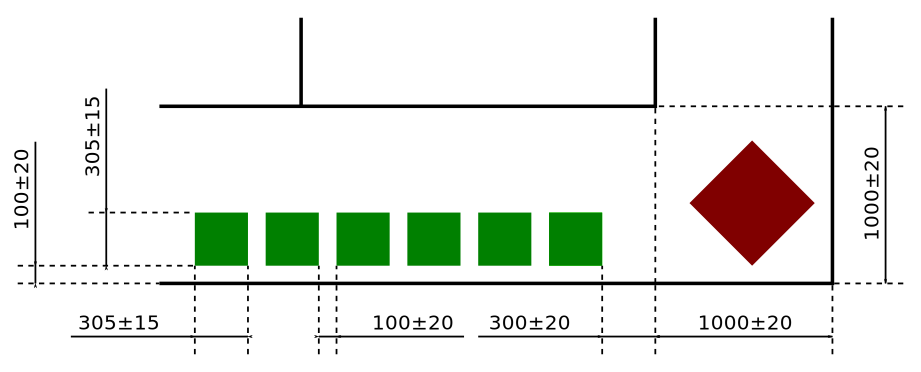
\includegraphics[width=\textwidth]{./images/token-position.pdf}
  \caption{Two perpendicular rows of four $200 \pm 15mm$ wide tokens are spaced evenly $300 \pm 20mm$ to the left and right of the robot's starting boundaries, along the arena walls.
    The tokens are placed $200 \pm 20mm$ away from each other, and $100 \pm 20mm$ from the arena wall.
           All dimensions are in millimetres.}
  \label{fig:token-position}
\end{figure}

\end{enumerate}

\clearpage
